%%%%%%%%%%%%%%%%%%%%%%%%%%%%%%%%%%%%%%%%%
% Beamer Presentation
% LaTeX Template
% Version 1.0 (10/11/12)
%
% This template has been downloaded from:
% http://www.LaTeXTemplates.com
%
% License:
% CC BY-NC-SA 3.0 (http://creativecommons.org/licenses/by-nc-sa/3.0/)
%
%%%%%%%%%%%%%%%%%%%%%%%%%%%%%%%%%%%%%%%%%

%----------------------------------------------------------------------------------------
%	PACKAGES AND THEMES
%----------------------------------------------------------------------------------------
\documentclass{beamer}

\mode<presentation> {

% The Beamer class comes with a number of default slide themes
% which change the colors and layouts of slides. Below this is a list
% of all the themes, uncomment each in turn to see what they look like.

%\usetheme{default}
%\usetheme{AnnArbor}
%\usetheme{Antibes}
%\usetheme{Bergen}
%\usetheme{Berkeley}
%\usetheme{Berlin}
%\usetheme{Boadilla}
%\usetheme{CambridgeUS}
%\usetheme{Copenhagen}
%\usetheme{Darmstadt}
%\usetheme{Dresden}
%\usetheme{Frankfurt}
%\usetheme{Goettingen}
%\usetheme{Hannover}
%\usetheme{Ilmenau}
%\usetheme{JuanLesPins}
%\usetheme{Luebeck}
\usetheme{Madrid}
%\usetheme{Malmoe}
%\usetheme{Marburg}
%\usetheme{Montpellier}
%\usetheme{PaloAlto}
%\usetheme{Pittsburgh}
%\usetheme{Rochester}
%\usetheme{Singapore}
%\usetheme{Szeged}
%\usetheme{Warsaw}

% As well as themes, the Beamer class has a number of color themes
% for any slide theme. Uncomment each of these in turn to see how it
% changes the colors of your current slide theme.

%\usecolortheme{albatross}
%\usecolortheme{beaver}
%\usecolortheme{beetle}
%\usecolortheme{crane}
%\usecolortheme{dolphin}
%\usecolortheme{dove}
%\usecolortheme{fly}
%\usecolortheme{lily}
%\usecolortheme{orchid}
%\usecolortheme{rose}
%\usecolortheme{seagull}
%\usecolortheme{seahorse}
%\usecolortheme{whale}
%\usecolortheme{wolverine}

%\setbeamertemplate{footline} % To remove the footer line in all slides uncomment this line
%\setbeamertemplate{footline}[page number] % To replace the footer line in all slides with a simple slide count uncomment this line

%\setbeamertemplate{navigation symbols}{} % To remove the navigation symbols from the bottom of all slides uncomment this line
}
%----------------------------------------------------------------------------------------
\usepackage{graphicx} % Allows including images
\usepackage{booktabs} % Allows the use of \toprule, \midrule and \bottomrule in tables
\setbeamerfont{caption}{size=\scriptsize}
\usepackage{hyperref}
\usepackage{listings}

%----------------------------------------------------------------------------------------
%	TITLE PAGE
%----------------------------------------------------------------------------------------
\title[]{ROS RVIZ} % The short title appears at the bottom of every slide, the full title is only on the title page
%----------------------------------------------------------------------------------------
\author{ARRA / AR2A} % Your name
\institute % Your institution as it will appear on the bottom of every slide, may be shorthand to save space
{
\textbf{A}dvancements for \textbf{R}obotics in \textbf{R}escue \textbf{A}pplications
}
\date{\today} % Date, can be changed to a custom date


%----------------------------------------------------------------------------------------
% if following command is uncommented
% there's a slide after each section
\AtBeginSection{\frame{\sectionpage}}

\setbeamertemplate{navigation symbols}{} % To remove the navigation symbols from the bottom of all slides uncomment this line
%----------------------------------------------------------------------------------------
\begin{document}
%----------------------------------------------------------------------------------------
\begin{frame}
\titlepage % Print the title page as the first slide
\end{frame}

%----------------------------------------------------------------------------------------
\begin{frame}
\frametitle{Overview} % Table of contents slide, comment this block out to remove it
\tableofcontents % Throughout your presentation, if you choose to use \section{} and \subsection{} commands, these will automatically be printed on this slide as an overview of your presentation
\end{frame}



%----------------------------------------------------------------------------------------
%	PRESENTATION SLIDES
%----------------------------------------------------------------------------------------
\section{Introduction}

\begin{frame}{RVIZ Introduction}	

	\begin{definition}
		\textbf{rviz (ROS Visualization)} is a 3D visualizer for displaying sensor data and state information from ROS. Using rviz, you can display live representations of sensor values coming over ROS Topics including camera data, infrared distance measurements, sonar data, and more. 
	
	\end{definition}
\end{frame}
%----------------------------------------------------------------------------------------

\subsection{RVIZ installation}
\begin{frame}[fragile]{RVIZ Prerequisites}	

	\begin{itemize}
		\item set up bash environment for ROS \\

			\lstinputlisting[frame=single, basicstyle=\footnotesize\ttfamily, language=C]{Shell/RVIZ_Installation_1.txt}
			note: after "source" follows a normal space	
		
		
		\item start roscore \\
			\lstinputlisting[frame=single, basicstyle=\footnotesize\ttfamily, language=C]{Shell/RVIZ_Installation_2.txt}
			
			
		\item start rviz \\
			\lstinputlisting[frame=single, basicstyle=\footnotesize\ttfamily, language=C]{Shell/RVIZ_Installation_3.txt}
		
	\end{itemize}

\end{frame}



%----------------------------------------------------------------------------------------

%----------------------------------------------------------------------------------------

\begin{frame}{RVIZ start screen}	

	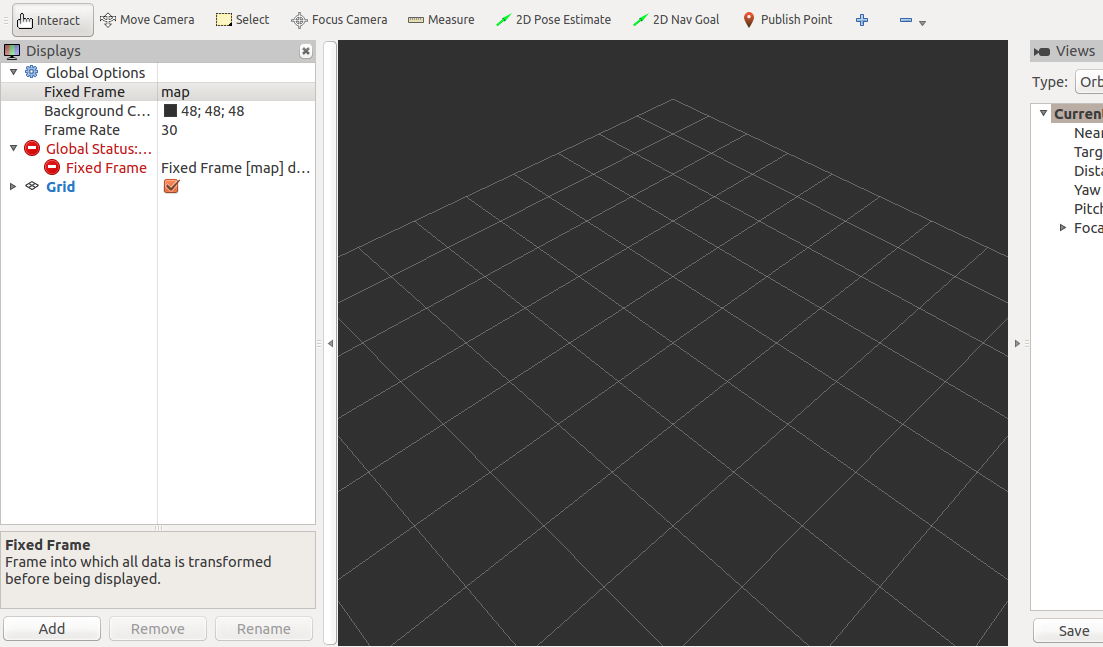
\includegraphics[width=\textwidth]{./Images/RVIZ_Start_Screen.png}

\end{frame}

%----------------------------------------------------------------------------------------

\section{RVIZ and Kinect}
\subsection{Kinect Driver}
\begin{frame}{Freenect (Microsoft Kinect Driver)}	

	\begin{itemize}
	
		\item install freenect: \\
			\lstinputlisting[frame=single, basicstyle=\footnotesize\ttfamily, language=C]{Shell/Freenect_1.txt}
		
		\item establish connection to Kinect \\
			\lstinputlisting[frame=single, basicstyle=\footnotesize\ttfamily, language=C]{Shell/Freenect_2.txt}
		
	\end{itemize}

\end{frame}

%----------------------------------------------------------------------------------------

\subsection{Setup}
\begin{frame}{RVIZ and KINECT Prerequisits}	

\begin{itemize}

	\item after initializing bash environment, start roscore and rviz
		\lstinputlisting[frame=single, basicstyle=\footnotesize\ttfamily, language=C]{Shell/Freenect_x.txt} 	
	
	
	\item establish connection to Kinect \\
		\lstinputlisting[frame=single, basicstyle=\footnotesize\ttfamily, language=C]{Shell/Freenect_2.txt} 
	
\end{itemize}
\end{frame}

%----------------------------------------------------------------------------------------

%----------------------------------------------------------------------------------------
\subsection{Example}
\begin{frame}{RVIZ - Frames}	

	\begin{itemize}
		\item Choose a Fixed Frame - for example camera\underline{ }depth\underline{ }optical\underline{ }frame
			
	\end{itemize}

	\begin{figure}[H]
		\centering
		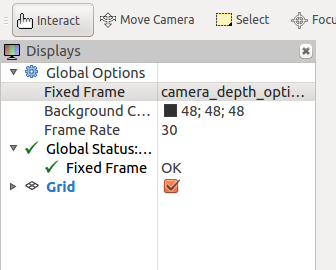
\includegraphics[scale=0.5]{./Images/RVIZ_Frame.png}
		\caption{choose a Fixed Frame}
		\label{fig:ros_add_frame}
	\end{figure}
\end{frame}

%----------------------------------------------------------------------------------------
\begin{frame}{RVIZ - Add an Image}	

	\begin{itemize}
		\item press button add - choose Image
			
	\end{itemize}

	\begin{figure}[H]
		\centering
		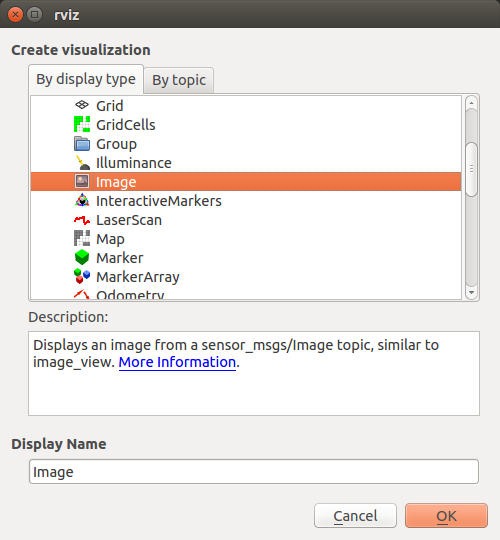
\includegraphics[scale=0.3]{./Images/Add_Image.png}
		\caption{add image }
		\label{fig:ros_add_image}
	\end{figure}

\end{frame}

%----------------------------------------------------------------------------------------
\begin{frame}{Kinect - Add a topic for the image}	

	\begin{itemize}
		\item select an image topic - for example: \\
			 
			\begin{itemize}
				\item /camera/depth/XXX
				\item /camera/rgb/XXX
				\item /camera/ir/XXX
			\end{itemize}
			
	\end{itemize}

	\begin{figure}[H]
		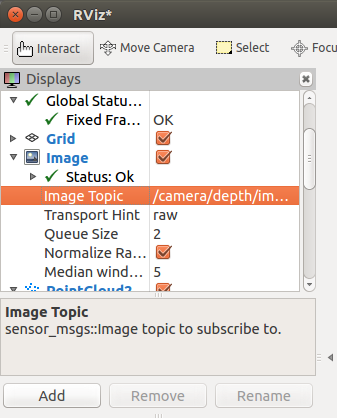
\includegraphics[scale=0.3]{./Images/Add_Image_Topic.png}
		\caption{select image topic}
		\label{fig:ros_image_topic}
	\end{figure}
		
\end{frame}

%----------------------------------------------------------------------------------------

%----------------------------------------------------------------------------------------
\begin{frame}{Kinect - Add a PointCloud2}	

\begin{itemize}
	\item Add PointCloud2
\end{itemize}

		\begin{figure}[H]
			\centering
			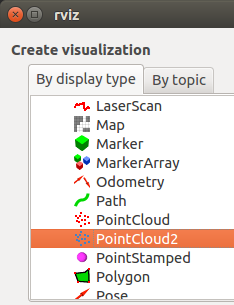
\includegraphics[scale=0.4]{./Images/Add_PointCloud2.png}
			\caption{add PointCloud2}
			\label{fig:ros_add_pointcloud}
		\end{figure}
		
\end{frame}

%----------------------------------------------------------------------------------------

\begin{frame}{RVIZ - Try different settings}	

	\begin{itemize}
		\item /camera/depth
		\item /camera/rgb
		\item try different settings: position, axis, transformer, color etc.
	\end{itemize}
\end{frame}

%----------------------------------------------------------------------------------------

%----------------------------------------------------------------------------------------
\subsection{Quick Start Commands}
\begin{frame}{RVIZ - quick start commands}	

	First start freenect driver (each command is two lines long):\\
	
			\lstinputlisting[frame=single, basicstyle=\footnotesize\ttfamily, language=C]{Shell/ShortCommandx.txt} 	

	\begin{itemize}
		
		\item compressed rgb image \\
			\lstinputlisting[frame=single, basicstyle=\footnotesize\ttfamily, language=C]{Shell/ShortCommand1.txt} 	
		
		\item compressed mono image \\
			\lstinputlisting[frame=single, basicstyle=\footnotesize\ttfamily, language=C]{Shell/ShortCommand2.txt} 	
		
	\end{itemize}
\end{frame}


\begin{frame}
\Huge{\centerline{The End}}
\end{frame}
%----------------------------------------------------------------------------------------
\end{document} 
%----------------------------------------------------------------------------------------